\section{Conclusiones}

El presente Trabajo Terminal tuvo como objetivo proponer e implementar un prototipo de aplicación que permita a la comunidad consultar los diferentes espacios con los que cuenta la Escuela Superior de Cómputo. Esto se logró con el uso de tecnologías disponibles para su consulta, tales como Mapbox que aunque no fue una tecnología utilizada fue de gran a ayuda para comprender el modelado de los polígonos con el fin de dibujar los edificios. La API de Google Maps como consulta también y diversos ejemplos de aplicaciones para el entorno de desarrollo de Apple.\\

Existen herramientas externas a las utilizadas por Apple que fueron de gran ayuda en la realización de este trabajo terminal. Un ejemplo de estas herramientas fue la utilización de \textbf{Pods} importados para mejorar la vista y funcionalidad de la aplicación. Librerías como \textbf{SVProgressHud} para la transición de carga, \textbf{Chameleon} para la utilización de colores, entre otras. \\

Con este trabajo damos un paso importante en la especialización que ambos integrantes queremos realizar en el desarrollo de aplicaciones móviles para dispositivos con sistema operativo iOS. De la misma manera satisfacemos parcialmente el gran interés por la ingeniería de software, sabiendo a donde dirigir nuestro futuro profesional.

\section{Resultados}

En esta sección se muestran los resultados obtenidos, los cuales comprenden los siguientes módulos:\\ \\

\begin{UClist} 
	\UCli Salones: En él, los actores son capaces de ubicar los edificios de la Escuela y obtener su información. De la misma manera se pueden ubicar los salones desde la pantalla de asignación de salones.
	\UCli Profesores: En este módulo, se puede obtener la lista de profesores registrados en la aplicación, así como el detalle de la información de contacto y ubicación.
	\UCli Unidades de Aprendizaje: Este módulo se compone de la lista de unidades de aprendizaje que se imparten o forman parte del plan de estudio de Ingeniería en Sistemas Computacionales en la Escuela Superior de Cómputo.
	\UCli Convocatorias de cursos: En este módulo se puede realizar la gestión de cursos que se ofertan en la ESCOM y que pueden ser difundidos por la misma escuela o algún centro dentro del Instituto que se relacione con la carrera de Ing. en Sistemas Computacionales.
	\UCli Convocarorias de movilidad:  En él, se muestran las dos convocatorias que se aperturan cada periodo escolar para realizar una movilidad acdémica ya sea dentro del país o en el extranjero.
\end{UClist} 

%\subsection{Módulo de Salones}
%
%En esta sección se puede observar el avance en la navegación y usabilidad de la aplicación como se muestra a continuación:
%
%%pantallas de la aplicación y si explicación
%
%\subsection{Módulo de Profesores}
%
%En esta sección se puede observar el avance en la navegación y usabilidad de la aplicación como se muestra a continuación:

%pantallas de la aplicación y si explicación

\section{Trabajo a Futuro}

Actualmente se está desarrollando el proyecto \textbf{CALMECAC} que será un sistema que integre todos los demás subsistemas con los que trabaja el Instituto y del que, como trabajadores del análisis y desarrollo del mismo, se pretende continuar con la generación de actualizaciones y mejoras al Trabajo Terminal, incluso la implementación de módulos no pretendidos en el alcance con la finalidad de ofrecerle a los alumnos la herramienta que integre los trámites y noticias qu le permitan obtener todo lo necesario durante su permanencia estudiantil en la Escuela Superior de Cómputo y exista la posibilidad de extenderse a todas las escuelas y centros de investigación del Instituto Politécnico Nacional. \\

Existe actualmente un Trabajo Terminal que busca implementar algunos de los módulos aquí propuestos y otros no tomados en cuenta dentro de nuestro alcance para la plataforma de desarrollo y sistema operativo Android. Se pretende colaborar con este equipo para retroalimentar los trabajos y llegar a ofrecer una herramienta que cubra con el mayor porcentaje posible de usuarios finales. \\

\section{Pruebas}

Se realizaron las pruebas de verificación en funcionalidad donde seguimos las trayectorias principales y alternativas de cada caso de uso dentro de la aplicación y se registró si existía algún fallo dentro de la usabilidad o si no existía fallo alguno. \\
Los resultados se muestran en la siguiente tabla: \\ \\

\cfinput{pruebas}

Como dispositivo físico de pruebas se utilizaron dos teléfono de la marca Apple, específicamente el modelo \textbf{A1784} con las siguientes características\footnote{Para fines de este trabajo no se consideran demás datos de hardware}: \\ \\

\begin{UClist} 
	\UCli Procesador Apple A10 Fusion de cuatros núcleos, dos de alto rendimiento y dos de alta eficiencia
	\UCli Memoria RAM de 3GB
	\UCli Memoria interna de 32GB para uno de los modelos y 256GB para el segundo
	\UCli Sistema Operativo iOS en su versión 11.4
	\UCli Conectividad NFC, WiFi 802.11 a/b/g/n/ac MIMO, Bluetooth 4.2, Redes 4G (LTE) \\
\end{UClist}

Durante el periodo de prueba se registró el pico de uso de los siguentes parámetros: \\ \\

\begin{UClist} 
	\UCli Uso del CPU en porcentaje
	\UCli Uso de la memoria RAM en MB
	\UCli Uso del disco en KB/s
	\UCli Uso de datos en la red mostrado en KB/s
	\UCli Impacto energético \\
\end{UClist}

Con pico de uso nos referimos al registro que el entorno de desarrollo Xcode recibe al momento de hacer las consultas dentro de la aplicación. Utilizando todos los módulos describimos en qué momento se registró el mayor porcentaje de uso de recursos dentro del teléfono de pruebas. \\

Al probar todos los módulos se encontró un uso máximo de CPU en 31\% como se muestra en la figura \ref{fig:cpu}

    \begin{figure}[h!]
	\begin{center}
		\fbox{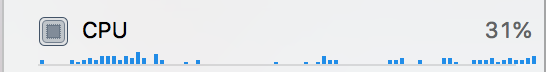
\includegraphics[width=.9\textwidth]{images/pruebas/cpu.png}}
		\caption{Uso máximo de CPU. \label{fig:cpu}}
	\end{center}
\end{figure}

Continuando con las pruebas, la mayor cantidad de memoria RAM utilizada durante el uso de la aplicación fue de 94.7MB como se muestra en la figura \ref{fig:memoria}

    \begin{figure}[h!]
	\begin{center}
		\fbox{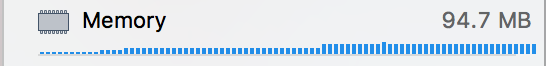
\includegraphics[width=.9\textwidth]{images/pruebas/memoria.png}}
		\caption{Uso máximo de memoria RAM. \label{fig:memoria}}
	\end{center}
\end{figure}

En lo que respecta al uso de memoria interna o disco duro se registraron 122 KB/s en el momento de más almacenamiento. Cabe mencionar que la aplicación no usa \textbf{CoreData} por lo que el almacenamiento puede ser temporal para que el consumo de datos sobre la red no se incremente. El uso se disco se puede ver en la figura \ref{fig:disco} 

    \begin{figure}[h!]
	\begin{center}
		\fbox{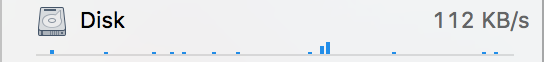
\includegraphics[width=.9\textwidth]{images/pruebas/disco.png}}
		\caption{Uso máximo de disco. \label{fig:disco}}
	\end{center}
\end{figure}

\newpage 
Al registrar el uso de datos sobre la red se encontró un punto máximo en la cantidad de 533 KB/s lo que nos indica que no exitió un alto de consumo de datos al hacer las consultas después de probar todos los módulos del sistema. El resultado se muestra en la figura \ref{fig:datos}

\begin{figure}[h!]
	\begin{center}
		\fbox{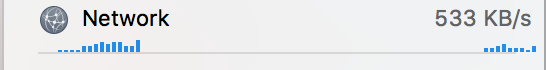
\includegraphics[width=.9\textwidth]{images/pruebas/datos.png}}
		\caption{Uso máximo de datos. \label{fig:datos}}
	\end{center}
\end{figure}

Por último se probó, ¿cuál sería el impacto energético que tiene nuestra aplicación sobre el teléfono? Si analizamos la figura \ref{fig:energia} vemos que únicamente cuando la barra azul se encuentra en su punto más alto se registra un alto impacto energético, cuando la barra se encuentra a la mitad del punto más alto y más abajo, se considera que tuvo un impacto enerético bajo. De acuerdo a la imagen concluimos que durante la consulta de todos los módulos del sistema se registró un alto impacto enerético en un 25\% de su uso y en el 75\% un bajo impacto.

\begin{figure}[h!]
	\begin{center}
		\fbox{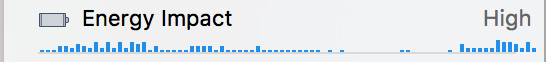
\includegraphics[width=.9\textwidth]{images/pruebas/energia.png}}
		\caption{Uso de energí. \label{fig:energia}}
	\end{center}
\end{figure}